\documentclass[10pt]{seminar} 

\renewcommand{\baselinestretch}{1}

\usepackage{amsmath}

\renewcommand{\printlandscape}{\special{landscape}}

\usepackage{ulem}



\input{seminar.bug}

%\usepackage{fancybox}

\usepackage{epsfig}

%\usepackage{times}


\usepackage{amssymb}

\usepackage{amscd}

\usepackage{graphics}

\usepackage{pstricks}

%\usepackage{chicago}

%\usepackage{fullpage}

\slideframe{none}

\begin{document}

\newtheorem{proposition}{Proposition}

\newtheorem{definition}{Definition}

\newtheorem{corollary}{Corollary}

\newtheorem{theorem}{Theorem}

\newtheorem{lemma}{Lemma}

\def\argmax{\mathop{\rm argmax}\limits}  


%\slideframe{Oval}

\sffamily 


\begin{slide}
\begin{center}

Determinants and quadratic forms
 \end{center}
 
 \newslide
 \small 
 
 Determinant rules
 
 \begin{itemize}
 \item The determinant of a triangular (square!) matrix, $\det \mathbf{A}$,  is the product of the entries on its diagonal
 \item In getting the matrix into triangular form using Gaussian elimination:
 \begin{itemize}
 \item If two rows are exchanged the determinant is multiplied by $-1$
 \item If a multiple of one row is subtracted from another the determinant is unchanged

 \end{itemize}
 \item A square matrix is singular if and only if its determinant is zero
 \item $\det (\lambda \mathbf{A})=\lambda^n \det {\mathbf{A}}$
 \item $\det (\mathbf{AB})=\det \mathbf{A} \det \mathbf{B}$
 \item $\det\mathbf{A}^{-1}={1\over {\det \mathbf{A}}}$
 \end{itemize}
 
 \newslide
 
The $2\times 2$ case
 
\ \\Let $$\mathbf{A}=\begin{bmatrix}a&b\\c&d
\end{bmatrix}$$
We write $$\det\mathbf{A}=\begin{vmatrix}a&b\\c&d
\end{vmatrix}$$ Reducing via Gaussian elimination we get
 $$\begin{bmatrix}a&b\\0&d-b{c\over a}
\end{bmatrix}$$
 The product of the diagonal entries is $$\det{\mathbf{A}}=ad-{{ab}}{c\over a} = ad-bc$$

\newslide
A longer example (let $k$ keep track of \# times rows switch)
$$\mathbf{A}=\begin{bmatrix}2& 3& 4\\2& 3& 7\\5& 8& 6
\end{bmatrix}$$

$$\begin{bmatrix}2& 3& 4\\0& 0& 3\\0& {1\over 2}& -4
\end{bmatrix} \hbox{ and }k=0$$

$$\begin{bmatrix}2& 3& 4\\0& {1\over 2}& -4\\0& 0& 3
\end{bmatrix} \hbox{ and }k=1$$

$$\det{\mathbf{A}}=(-1)^k (3)=-3$$

\newslide
What is a determinant?

\ \\For $2\times 2$ matrices they have a natural interpretation: 

\begin{center}
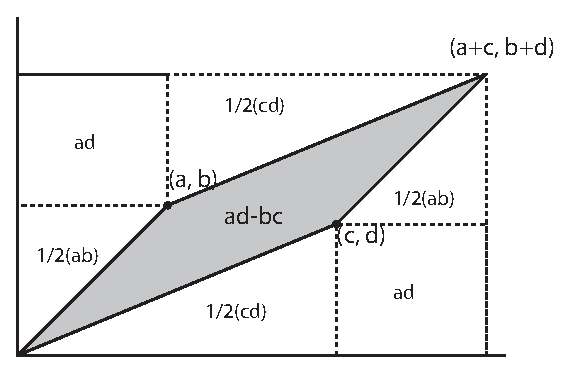
\epsfig{file=parallelogram.eps, scale=.75}
\end{center}

The area of the parallelogram is $$|(a+c)(b+d)-2ad-ab-cd|=|ab+ad+bc+cd-2ad-ab-cd|=|ad-bc|$$
\newslide

Transposition

\ \\The transpose of a matrix, $\mathbf{A}^T$ is the matrix whose rows are the columns of $\mathbf{A}$

$$\begin{bmatrix}
1 & 2& 3& 4\\
0& 1& 0& 1\\
5& 5& 5& 5
\end{bmatrix}^T =
\begin{bmatrix}
1 &0 & 5\\
2& 1& 5\\
3& 0& 5\\
4& 1& 5
\end{bmatrix}
$$

\newslide

Last class we discussed how the rank of a matrix could be computed by looking at the maximal number of linearly independent \textit{rows} or \textit{columns}

\ \\This implies that $$\hbox{rank } \mathbf{A}^T=\hbox{rank } \mathbf{A}$$

\ \\We can get more than this:

$$\det \mathbf{A}^T=\det \mathbf{A}$$

\ \\(For the $2\times 2$ case, this is obvious)

\newslide
Inner products

If $\mathbf{x}$ and $\mathbf{y}$ are both $n-$vectors, then the product $\mathbf{x}^T\mathbf{y}$ is the scalar 
$$x_1y_1+x_2y_2+...+x_ny_n$$
This is called the \textit{inner product} or \textit{dot product} or \textit{scalar product} of $\mathbf{x}$ and $\mathbf{y}$ and is written $$\mathbf{x}^T \mathbf{y}\hbox{ or }\mathbf{x}\cdot \mathbf{y} \hbox{ or } \langle\mathbf{x}\mathbf{y}\rangle$$

\ \\Example: Let $\mathbf{p}$ be a vector of prices of $n$ goods and $\mathbf{x}$ be a vector of quantities of those $n$ goods; then $\mathbf{x}\cdot \mathbf{p}=\sum_{i=1}^n p_i x_i$ is total expenditure

\newslide
Length and  distance

\ \\As $\mathbf{x}\cdot \mathbf{x}=\sum_{i} x_i^2$, it follows that the distance between the origin $\mathbf{0}$ and $\mathbf{x}$ is $\sqrt{\mathbf{x}\cdot\mathbf{x}}$

\ \\We call $\sqrt{\mathbf{x}\cdot\mathbf{x}}$ the \textit{length, magnitude}, or \textit{norm} of $\mathbf{x}$, and denote it $||\mathbf{x}||$

\begin{itemize}
\item $||\mathbf{a}||>0$ if $\mathbf{a}\not=0$
\item $|\mathbf{a}\cdot \mathbf{b}|\leq ||\mathbf{a}|| ||\mathbf{b}||$ (Cauchy-Schwarz inequality)
\item $||\mathbf{a}+\mathbf{b}||\leq ||\mathbf{a}||+||\mathbf{b}||$ (Triangle inequality)
\end{itemize}

(We'll prove the latter two statements shortly)

\newslide
Orthogonality

\ \\Let $\mathbf{a}$ and $\mathbf{b}$ be two $n-$vectors; then $\mathbf{a}$ is \textit{orthogonal} to $\mathbf{b}$ if $\mathbf{a}\cdot \mathbf{b}=0$

\begin{center}
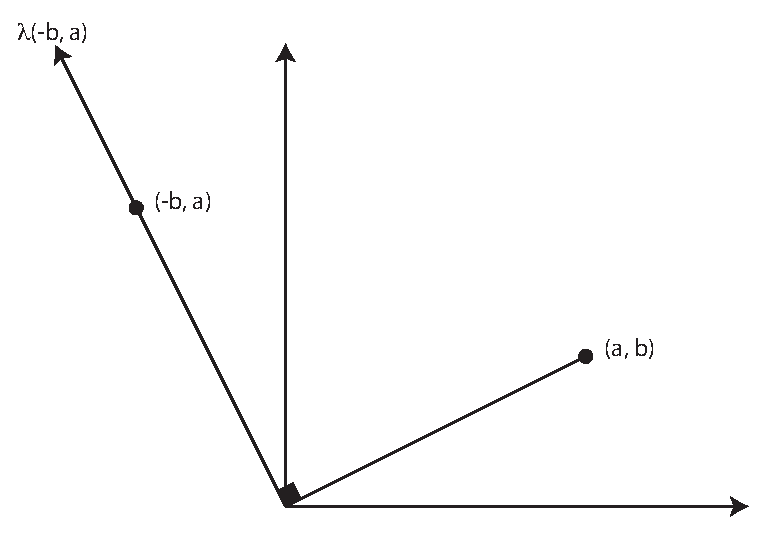
\epsfig{file=orthogonal.eps, scale=.7}
\end{center}

\newslide
The geometry of dot products more generally

\ \\$\mathbf{a} \cdot \mathbf{b}=||\mathbf{a}||||\mathbf{b}||\cos \theta$, where $\theta $ is the angle between $\mathbf{a}$ and $\mathbf{b}$

\ \\$\cos 90^\circ =0$  and so $\mathbf{a} \cdot \mathbf{b}=0$ if they're orthogonal
\ \\$\cos 0^\circ =1$ and so $\mathbf{a} \cdot \mathbf{a} = ||\mathbf{a}|| || \mathbf{a}||$
\ \\$\cos \theta\in [-1, 1]$ for all angles $\theta$


\ \\Using this, the Cauchy-Schwarz inequality is immediate:

$|\mathbf{a}\cdot \mathbf{b}|=||\mathbf{a}||   ||\mathbf{b}||  |\cos \theta |\leq ||\mathbf{a}||||\mathbf{b}||$


\newslide

The triangle inequality follows from the Cauchy-Schwarz inequality:

\ \\We want to prove $||\mathbf{a}+\mathbf{b}||\leq ||\mathbf{a}||+||\mathbf{b}||$

\ \\ $$\begin{array}{rcl}||\mathbf{a}+\mathbf{b}||^2&=&\langle\mathbf{a}+\mathbf{b}, \mathbf{a}+\mathbf{b}\rangle\\

&=&\langle \mathbf{a}, \mathbf{a}\rangle +2 \langle \mathbf{a}, \mathbf{b}\rangle+\langle \mathbf{b}, \mathbf{b}\rangle\\
&\leq &\langle \mathbf{a}, \mathbf{a}\rangle +2 |\langle \mathbf{a}, \mathbf{b}\rangle|+\langle \mathbf{b}, \mathbf{b}\rangle\\
&\leq &\langle \mathbf{a}, \mathbf{a}\rangle +2 || \mathbf{a}||  ||\mathbf{b}||+\langle \mathbf{b}, \mathbf{b}\rangle \hbox{ (Cauchy-Schwarz)}\\
&= &||\mathbf{a}||^2 +2 || \mathbf{a}||  ||\mathbf{b}||+ ||\mathbf{b}||^2\\
&=&(||\mathbf{a}||+||\mathbf{b}||)^2
\end{array}
$$

Taking a square root on each side we get $$||\mathbf{a}+\mathbf{b}||\leq ||\mathbf{a}||+||\mathbf{b}||  \hspace{.05in}\Box$$ 

\newslide

Quadratic forms and symmetric matrices

\begin{itemize}
\item A \textit{quadratic form} is a homogenous quadratic polynomial in $n$ variables
\begin{itemize}
\item A \textit{homogeneous polynomial} is a polynomial whose nonzero terms all have the same degree: in words, the sum of the exponents of each term is constant
\item A \textit{homogenous quadratic polynomial} is a polynomial whose terms all have degree 2
\item $a x^2$
\item $ax^2+bxy+cy^2$
\item $a x^2+b y^2+c z^2+d xy+e xz+f yz$ (with coefficients $a, b, c, d, e, f$)
\end{itemize}

\end{itemize}
\newslide

Consider the two variable quadratic form
$$q(x, y)=ax^2+bxy+cy^2$$
Using our techniques from last class we know we can write $$q(x, y)=\mathbf{z}^T\mathbf{A}\mathbf{z}$$ where $$\mathbf{z}=\begin{bmatrix}
x\\y
\end{bmatrix} \hbox{ and }\mathbf{A}=
\begin{bmatrix}
a & s \\
t& c
\end{bmatrix} 
$$
with $s+t=b$

\ \\If we impose the condition that $\mathbf{A}$ is symmetric (so that $\mathbf{A}=\mathbf{A}^T$, or $a_{ij}=a_{ji}$ for all $i, j$) then we have $s=t={b\over 2}$
 
 \ \\There is therefore a unique symmetric matrix $\mathbf{A}$ satisfying $q(x, y)=\mathbf{z}^T\mathbf{A}\mathbf{z}$

\newslide

This generalizes:

\ \\Let $q(\mathbf{x})$ be a quadratic form in $n$ variables, $x_1, ..., x_n$

\ \\Then $q(\mathbf{x})$ is equivalent to the expression 

$$\mathbf{x}^T\mathbf{A}\mathbf{x}$$ for a unique symmetric $n\times n$ matrix $\mathbf{A}$ and $\mathbf{x}^T=[x_1, x_2, ..., x_n]$

\ \\Takeaway point: A symmetric $\mathbf{A}$ is uniquely determined by the coefficients in  $q(\mathbf{x})$

\newslide

Definite and semidefinite quadratic forms

\ \\For a given quadratic form $q(\mathbf{x})$ we can ask whether $q(\mathbf{x})>0$ (or less stringently, $q(\mathbf{x})\geq 0$) for every non-zero $\mathbf{x}$

\ \\If  $q(\mathbf{x})>0$ for every non-zero $\mathbf{x}$ then $q(\mathbf{x})$ is \textit{positive definite}

\begin{itemize}
\item Example $q(\mathbf{x}) = x_1^2+x_2^2+...+x_n^2$
\end{itemize}

\ \\If  $q(\mathbf{x})\geq 0$ for every $\mathbf{x}$ then $q(\mathbf{x})$ is \textit{positive semidefinite}

\begin{itemize}
\item Example $q(\mathbf{x}) = x_1^2+x_2^2+x_3^2-2x_2x_3$
\begin{itemize}
\item $q(\mathbf{x}) = x_1^2+(x_2-x_3)^2 \geq 0$ but $q(0, 1, 1)=0$
\end{itemize}
\end{itemize}

\newslide
More on positive (and negative) definiteness

\ \\If  $q(\mathbf{x})<0$ for every non-zero $\mathbf{x}$ then $q(\mathbf{x})$ is \textit{negative definite}

\ \\If  $q(\mathbf{x})\leq 0$ for every $\mathbf{x}$ then $q(\mathbf{x})$ is \textit{negative semidefinite}

\ \\Most  quadratic forms are neither positive nor negative semidefinite

\ \\Example: $q(x, y)=xy$
\begin{itemize}
\item $q(1, 1)>0$
\item $q(1, -1)<0$
\end{itemize}

\newslide
Testing quadratic forms

\ \\We can test if a quadratic form is positive (negative) (semi)definite by testing the associated symmetric matrix $\mathbf{A}$ that satisfies $q(\mathbf{x})=\mathbf{x}^T\mathbf{A}\mathbf{x}$

\ \\If $\mathbf{A}$ is $2\times 2$, and recall, $\mathbf{A}=\begin{bmatrix}a& c\\c& d\end{bmatrix}$, then:

\begin{itemize}
\item $\mathbf{A}$ is PD iff $a, d>0$ and $\det \mathbf{A}>0$
\item $\mathbf{A}$ is PSD iff  $a, d\geq0$ and $\det \mathbf{A}\geq 0$
\item $\mathbf{A}$ is ND iff $a, d<0$ and $\det \mathbf{A}>0$
\item $\mathbf{A}$ is NSD iff  $a, d\leq $ and $\det \mathbf{A}\geq 0$
\end{itemize}

\newslide
Testing matrices for ``definiteness" is something we do a lot of in optimization\footnote{Taylor's Theorem implies the second-order behavior of smooth functions of several variables can be described by the quadratic form of the function's Hessian, which is a symmetric matrix of the function's partial derivatives}

\ \\Definitions

\begin{itemize}
\item A \textit{submatrix} of $\mathbf{A}$ is a matrix obtained by deleting some rows and columns of $\mathbf{A}$
\item A \textit{principal submatrix} of a square $\mathbf{A}$ is a submatrix obtained by requiring that if the $k$th row is deleted then the $k$th column is deleted
\item A \textit{leading principal submatrix} of  $\mathbf{A}$ is a principal submatrix obtained by deleting the last $m$ rows and columns for some $m<n$
\end{itemize}

\newslide

$$\mathbf{A}=\begin{bmatrix}
a& b& c\\
d& e& f\\
g& h& i
\end{bmatrix}$$

\ \\The 7 principal submatrices are:

$$\begin{bmatrix}
a
\end{bmatrix}
\begin{bmatrix}
e
\end{bmatrix}
\begin{bmatrix}
i
\end{bmatrix}
\begin{bmatrix}
a & b\\ d& e
\end{bmatrix}
\begin{bmatrix}
a & c\\g& i
\end{bmatrix}
\begin{bmatrix}
e& f\\h& i
\end{bmatrix}
\begin{bmatrix}
a& b& c\\
d& e& f\\
g& h& i
\end{bmatrix}$$
\ \\The 3 leading principal submatrices are:

$$\begin{bmatrix}
a
\end{bmatrix}
\begin{bmatrix}
a & b\\ d& e
\end{bmatrix}
\begin{bmatrix}
a& b& c\\
d& e& f\\
g& h& i
\end{bmatrix}$$

\newslide
Minors

\begin{itemize}
\item A \textit{minor} of $\mathbf{A} $ is the determinant of a submatrix of $\mathbf{A} $
\item A \textit{ principal minor} of $\mathbf{A} $ is the determinant of a principal submatrix of $\mathbf{A} $
\item A \textit{leading principal minor} of $\mathbf{A} $ is the determinant of a leading principal submatrix of $\mathbf{A} $
\end{itemize}
\vspace{.1in}

Test for positive definiteness: An $n\times n$ symmetric matrix $\mathbf{A}$ is positive definite if and only if its leading principal minors are all positive

\vspace{.1in}

Test for positive semidefiniteness: An $n\times n$ symmetric matrix $\mathbf{A}$ is positive semidefinite if and only if its  principal minors are all non-negative

  \vspace{.1in}
  
  (Test for negative (semi)definiteness by applying above conditions to $-\mathbf{A} $)
  
  \newslide
  
  Least squares estimation
  
  \ \\Suppose you have data consisting of $2$ observations on three variables, $(y, x_1, x_2)$; you want to find a function of the form $$y=\beta_1x_1+\beta_2x_2$$ that fits the data best: $\beta_1$ and $\beta_2$ minimize the expression $$q(\beta_1, \beta_2)=\sum_{i=1}^2 (y_i-\beta_1x_{i1}-\beta_2x_{i2})^2$$
  
\ \\  Let $$\mathbf{y}=
\begin{bmatrix}y_1\\y_2
\end{bmatrix}
\mathbf{X}=
\begin{bmatrix}x_{11}& x_{12}\\x_{21}& x_{22}
\end{bmatrix}
\mathbf{b}=
\begin{bmatrix}\beta_1\\ \beta_2
\end{bmatrix}
$$

Note that $$\mathbf{Xb}=\begin{bmatrix}\beta_1x_{11}+\beta_2 x_{12}\\\beta_1x_{21}+\beta_2 x_{22}
\end{bmatrix}$$
  
  
  \newslide
  
  $$\mathbf{y}=
\begin{bmatrix}y_1\\y_2
\end{bmatrix}  \mathbf{Xb}=\begin{bmatrix}\beta_1x_{11}+\beta_2 x_{12}\\\beta_1x_{21}+\beta_2 x_{22}
\end{bmatrix}$$
  
  
\ \\We can rewrite $q(\beta_1, \beta_2)=\sum_{i=1}^2 (y_i-\beta_1x_{i1}-\beta_2x_{i2})^2$ as 
  
  $$q(\mathbf{b})=\langle \mathbf{y}-\mathbf{Xb}, \mathbf{y}-\mathbf{Xb}\rangle$$
  

\newslide
  $$q(\mathbf{b})=\langle \mathbf{y}-\mathbf{Xb}, \mathbf{y}-\mathbf{Xb}\rangle$$

Finding $\mathbf{b}=\begin{bmatrix} \beta_1 \\ \beta_2\end{bmatrix}$  to minimize $q$ is an optimization problem in 2 variables


 $$q(\mathbf{b})=\langle\mathbf{y}, \mathbf{y} \rangle +\langle \mathbf{Xb}, \mathbf{Xb} \rangle -2\langle \mathbf{y}, \mathbf{Xb} \rangle$$

$$q(\beta_1, \beta_2)= y_1^2+y_2^2$$ $$+ (\beta_1 x_{11}+\beta_2 x_{12})^2+(\beta_1 x_{21}+\beta_2 x_{22})^2 $$ $$-2 \left(y_1 (\beta_1 x_{11}+\beta_2 x_{12})\right)-2\left(y_2 (\beta_1 x_{21}+\beta_2 x_{22})\right)$$


\newslide

 $$q(\mathbf{b})=\langle\mathbf{y}, \mathbf{y} \rangle +\langle \mathbf{Xb}, \mathbf{Xb} \rangle -2\langle \mathbf{y}, \mathbf{Xb} \rangle$$

$$q(\beta_1, \beta_2)= y_1^2+y_2^2$$ $$+ (\beta_1 x_{11}+\beta_2 x_{12})^2+(\beta_1 x_{21}+\beta_2 x_{22})^2 $$ $$-2 \left(y_1 (\beta_1 x_{11}+\beta_2 x_{12})\right)-2\left(y_2 (\beta_1 x_{21}+\beta_2 x_{22})\right)$$

Differentiating with respect to $\beta_1, \beta_2$:

$${\partial q\over \partial \beta_1}=2(\beta_1 x_{11}+\beta_2x_{12})x_{11}+2(\beta_1 x_{21}+\beta_2x_{22})x_{21}-2(y_1x_{11}+y_2 x_{21})=0$$

$${\partial q\over \partial \beta_2}=2(\beta_1 x_{11}+\beta_2x_{12})x_{12}+2(\beta_1 x_{21}+\beta_2x_{22})x_{22}-2(y_1x_{12}+y_2 x_{22})=0$$
\newslide

$${\partial q\over \partial \beta_1}=2(\beta_1 x_{11}+\beta_2x_{12})x_{11}+2(\beta_1 x_{21}+\beta_2x_{22})x_{21}-2(y_1x_{11}+y_2 x_{21})=0$$

$${\partial q\over \partial \beta_2}=2(\beta_1 x_{11}+\beta_2x_{12})x_{12}+2(\beta_1 x_{21}+\beta_2x_{22})x_{22}-2(y_1x_{12}+y_2 x_{22})=0$$

Moving back to matrix notation we can write these equations as 


$$ \mathbf{X}^T\mathbf{X} \mathbf{b}= \mathbf{X}^T\mathbf{y}  $$

Assuming $\mathbf{X}^T\mathbf{X} $ has full rank (is invertible), this is an equation of the form $\mathbf{Ax}=\mathbf{y}$; thus the least squares solution is:

$$ \mathbf{b}^*=  (\mathbf{X}^T\mathbf{X})^{-1}\mathbf{X}^T\mathbf{y}  $$
\newslide


    Playing with our result  $$\mathbf{b}^*=(\mathbf{X}^T \mathbf{X})^{-1}\mathbf{X}^T\mathbf{y}$$ 
\begin{center}
\begin{tabular}{c|c|c|c}

Country & Life expectancy & Per Cap GDP& Pop density \\ \hline \hline

USA & 78&48 &85\\
Russia & 70&17 &21 \\
Brazil  &73 &12 & 62
\end{tabular}
    \end{center}
$$    \mathbf{X}= \begin{bmatrix} 48&85\\17&21\\12&62
\end{bmatrix} \hbox{ and }
  \mathbf{y}= \begin{bmatrix} 78\\70\\73
\end{bmatrix}
$$

If we calculate $(\mathbf{X}^T \mathbf{X})^{-1}\mathbf{X}^T\mathbf{y}$ using the above matrices we get $\mathbf{b}^*=\begin{bmatrix} 0.3128 \\0.9561
\end{bmatrix}
\hbox{ and so  Life expectancy = .3128 GDP + .9561 Density} 
$ fits the data best, in the sense of minimizing $\sum_{i=1}^3(\hbox{Life expectancy}_i-b_1^*\hbox{GDP}_i-b_2^*\hbox{density}_i)^2$
    
 \end{slide}
 
 \end{document}





Suppose that $\mathbf{b}^*$ is a 2-vector $\begin{bmatrix} \beta^*_1 \\ \beta^*_2\end{bmatrix}$ 

that solves $$\mathbf{X}^T(\mathbf{y}-\mathbf{Xb}^*)=\mathbf{0}$$  



We can rewrite $$\mathbf{y}-\mathbf{Xb}=\mathbf{y}-\mathbf{Xb}^*+\mathbf{X}(\mathbf{b}^*-\mathbf{b})$$ and 
$$\langle \mathbf{y}-\mathbf{Xb}, \mathbf{y}-\mathbf{Xb}\rangle=\langle \mathbf{y}-\mathbf{Xb}^*+\mathbf{X}(\mathbf{b}^*-\mathbf{b}),\mathbf{y}-\mathbf{Xb}^*+\mathbf{X}(\mathbf{b}^*-\mathbf{b})\rangle$$
$$=\langle \mathbf{y}-\mathbf{Xb}^*,\mathbf{y}-\mathbf{Xb}^*\rangle +\langle \mathbf{X}(\mathbf{b}^*-\mathbf{b}), \mathbf{X}(\mathbf{b}^*-\mathbf{b})\rangle +2 \langle \mathbf{y}-\mathbf{Xb}^*, \mathbf{X}(\mathbf{b}^*-\mathbf{b})\rangle$$
\newslide

Note that 
$$\langle\mathbf{y}-\mathbf{Xb}^*, \mathbf{X}(\mathbf{b}^*-\mathbf{b})\rangle$$

$$=\sum_{i=1}^2(y_i-\beta^*_1x_{i1}-\beta^*_2x_{i2}) (x_{i1} (\beta_1^*-\beta_1)+x_{i2}(\beta_2^*-\beta_2))=0$$
    This is because $$\mathbf{X}^T(\mathbf{y}-\mathbf{Xb}^*)=\begin{bmatrix}\sum_{i=1}^2 x_{i1}(y_i-\beta^*_1x_{i1}-\beta^*_2x_{i2}) \\ \sum_{i=1}^2  x_{i2}(y_i-\beta^*_1x_{i1}-\beta^*_2x_{i2})\end{bmatrix}=\begin{bmatrix}0\\0
    \end{bmatrix}$$
    \newslide
    Returning to our previous result we have that 
    
    $$q(\mathbf{b})=\langle \mathbf{y}-\mathbf{Xb}, \mathbf{y}-\mathbf{Xb}\rangle=\langle \mathbf{y}-\mathbf{Xb}^*+\mathbf{X}(\mathbf{b}^*-\mathbf{b}),\mathbf{y}-\mathbf{Xb}^*+\mathbf{X}(\mathbf{b}^*-\mathbf{b})\rangle$$
$$=\langle \mathbf{y}-\mathbf{Xb}^*,\mathbf{y}-\mathbf{Xb}^*\rangle +\langle \mathbf{X}(\mathbf{b}^*-\mathbf{b}), \mathbf{X}(\mathbf{b}^*-\mathbf{b})\rangle +2 \langle \mathbf{y}-\mathbf{Xb}^*, \mathbf{X}(\mathbf{b}^*-\mathbf{b})\rangle$$


$$q(\mathbf{b})=\langle \mathbf{y}-\mathbf{Xb}^*,\mathbf{y}-\mathbf{Xb}^*\rangle +\langle \mathbf{X}(\mathbf{b}^*-\mathbf{b}), \mathbf{X}(\mathbf{b}^*-\mathbf{b})\rangle $$

\ \\Since the columns of $\mathbf{X}$ are linearly independent, $\mathbf{X}^T\mathbf{X}$ (a $2\times 2$ symmetric matrix) is positive definite and invertible (a result in your book)

\ \\This implies that $\langle \mathbf{X}(\mathbf{b}^*-\mathbf{b}), \mathbf{X}(\mathbf{b}^*-\mathbf{b})\rangle = (\mathbf{b}^*-\mathbf{b})^T\mathbf{X}^T\mathbf{X}(\mathbf{b}^*-\mathbf{b})$ is always positive
    
    \ \\Which implies that $q(\mathbf{b})$ is minimized at $\mathbf{b}=\mathbf{b}^*$
    



